\documentclass{article}
\usepackage{graphicx}
\usepackage[export]{adjustbox}
\usepackage[spanish]{babel}
\usepackage[utf8]{inputenc}
\usepackage{indentfirst}
\usepackage{float}
\usepackage{lastpage}
\usepackage{subfig}
\usepackage{booktabs}
\usepackage{pgfplots}
\usepackage{listings}
\usepackage{fancyhdr}
\setlength{\parskip}{1ex}
\usepackage{amssymb,amsmath}
\usepackage[hidelinks]{hyperref} 
\graphicspath{{C:/Users/Gustavo/Documents/Electrónica/7.- Semestre/Control/Reportes\P2}}
\usepackage[left=2.5cm,
			top=2.5cm,
			right=2.5cm,
			bottom=3cm]{geometry}
\lstset{language=Scilab, breaklines=true, basicstyle=\footnotesize}
\lstset{numbers=left, numberstyle=\tiny, stepnumber=2, numbersep=-8pt}

%Materia y maestro
\newcommand{\materia}{\uppercase{Control I}}
\newcommand{\maestro}{\uppercase{M.C. Gerardo Marx Chávez-Campos}}

%Tipo de documento y nombres de tema
\newcommand{\tipoDoc}{\uppercase{}} %TAREA, REPORTE DE LABORATORIO,
\newcommand{\nombreDoc}{\uppercase{Reporte Práctica No. 2}} 
\newcommand{\docNum}{}
\newcommand{\subNombreDoc}{\uppercase{Poles and zeros found by Inspection}}

%Alumnos y fecha
\newcommand{\alumnos}{Gustavo Martínez Mondragón \\
	Carlos Alberto Del Portillo Malandra}
\newcommand{\fecha}{\uppercase{13 de noviembre de 2017}}



\begin{document}
	%Cabezal del membrete
	\begin{center}
		
\includegraphics[scale=.5]{encabezado}
		\vspace{.3cm}
		\hrule height2.5pt
		\vspace{.1cm}
		\hrule height1pt
		\vspace{.3cm}
		\huge INSTITUTO TECNOLÓGICO DE MORELIA \\
		\vfill
		\large DIVISIÓN DE ESTUDIOS PROFESIONALES  \\
		\vfill
		\large  DEPARTAMENTO DE INGENIERÍA ELECTRÓNICA \\ 
		\vfill
		\Large \textbf \materia \\
		\vfill
		\textbf{\tipoDoc} \\
		\vfill 
		\LARGE  \textbf{ \nombreDoc  \, \docNum: \\ \subNombreDoc} \\
		\vfill
		\large PRESENTA(N): \\
		\large  \textbf{\alumnos} \\
		\vfill
		\large PROFESOR: \\
		\Large \textbf{\maestro }
		\vfill 
	\end{center}
	\begin{flushleft}
		MORELIA, MICHOACÁN \hfill \uppercase{\fecha}
	\end{flushleft}
	
	
	
	\thispagestyle{empty} 
	\newpage
	\tableofcontents
	\thispagestyle{empty}
	\newpage
	\pagestyle{fancy}
	\lhead{Control I}
	\chead{Práctica No. 2}
	\rhead{\alumnos}
	\lfoot{Depto. de Ingeniería Electrónica}
	\cfoot{\thepage\ de \pageref{LastPage}}
	\rfoot{Instituto Tecnológico de Morelia}
	\section{Introducción}
	Para cualquier sistema en control necesitamos cierta estabilidad en el mismo esto quiere decir que si tenemos una entrada $ V_{in} $ deberíamos tener una salida $ V_{out} $ que será el resultado de la multiplicación de una \textit{\textbf{función de transferencia}} por la entrada.
	
	\begin{equation}
	V_{out}=V_{in}G(s)
	\end{equation}
	
	Entonces tenemos que nuestra función de trasferencia del sistema, G(s), es igual a la salida sobre nuestra entrada.
	\begin{equation}
	G(s)=\frac{V_{out}}{V_{in}}
	\end{equation}
	
	Las polos y ceros se expresan en la función de transferencia de la siguiente manera:
	
	\begin{equation}
	G(s)=G_0\frac{(1+s/w_{z1})}{(1+s/w_{p1})}
	\label{transfun}
	\end{equation}
	
	Donde:
	$ w_{z1} $= cero de la función de transferencia\\
	
	$ w_{p1} $= polo de la función de transferencia\\
	
	Los polos de la función de trasferencia deben ser reales o pares de complejos conjugados por lo mismo las partes reales de todos los polos deben ser negativas para que el sistema sea estable
	Ceros. \\
	
	El valor(es) para Z donde el numerador de la función de trasferencia sea igual a cero.
	Polos. \\
	
	El valor(es) para Z  donde el denominador de la función de transferencia igual a cero.\\
	
	
	El objetivo de la práctica es encontrar la función de transferencia de un circuito RL, por medio del método de inspección para obtener todos sus elementos: polos, ceros y $ G_0 $. 
	
	Tras hacer ese análisis teórico, se utilizará LTspice para simularlo y comparar posteriormente con los resultados obtenidos en el laboratorio, donde se efectuará un barrido de frecuencia y se encontrará el valor del factor de tiempo Tau ($ \tau $).
	
	
	\section{Metodología}
	
	A continuación en la figura \ref{fig:circ} se muestra el circuito que se analizará.
	
	\begin{figure}[H]
		\centering
		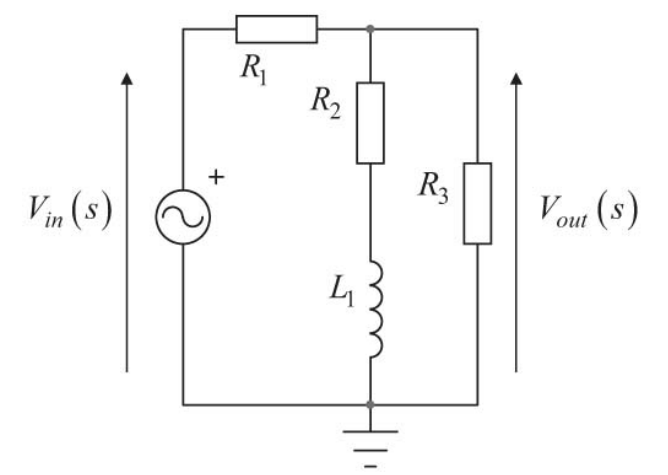
\includegraphics[scale=0.5]{circ}
		\caption{Diagrama del circuito RL.}
		\label{fig:circ}
	\end{figure}
	
	
	\subsection{Desarrollo teórico}
	\subsubsection{Método de Inspección}
	
	Lo primero que se debe encontrar de la función de transferencia \eqref{transfun} es $ G_0 $, el \textit{\textbf{bias-point}} o punto en DC, donde la frecuencia \textit{s=0}. AL hacer esto, el inductor se convierte en un corto circuito y obtenemos que:
	
	\begin{equation}
	V_{out}=V_{in}\frac{R_2||R_3}{(R_2||R_3)+R_1}\quad G_0=\frac{V_{out}(s)}{V_{in}(s)}=\frac{R_2||R_3}{(R_2||R_3)+R_1}
	\label{bias}
	\end{equation}
	
	Para obtener el cero de nuestro circuito, se toma la rama del circuito en el que se tiene un elemento afectado por la frecuencia, en este caso es el inductor, y se iguala a cero; al hacer está consideración, se puede decir que se llega a un punto donde la frecuencia es infinita. Entonces tenemos en el dominio de Laplace que:
	
	\begin{equation}
	R_2+sL=0
	\label{cerocirc}
	\end{equation}
	
	Los ceros están expresados de la forma
	
	\begin{equation}
	1+\frac{s}{w_{z1}}=0
	\label{cerogen}
	\end{equation}
	
	Por lo que tenemos que dejar la ecuación \eqref{cerocirc} lo más parecida a \eqref{cerogen}, por lo que dividimos todo entre $ R_2 $:
	
	\begin{equation}
	1+\frac{sL}{R_2}=0
	\label{cerocirc2}
	\end{equation}
	
	Entonces igualamos \eqref{cerogen} con \eqref{cerocirc2} para obtener el cero:
	
	\begin{equation}
	\begin{split}
	1+\frac{sL_1}{R_2}=	1+\frac{s}{w_{z1}}\\
	\frac{L}{R_2}=1-1+\frac{s}{sw_{z1}}\\
	\frac{L}{R_2}=\frac{1}{w_{z1}}\\
	w_{z1}=\frac{R_2}{L} \label{zero}
	\end{split}
	\end{equation}
	
	Para encontrar el polo del circuito, debemos encontrar el inverso de la constante de tiempo de nuestro circuito, es decir:
	
	\begin{equation}
	\begin{split}
	\tau=\frac{L}{R}\\
	\frac{1}{\tau}=\frac{R}{L}
	\end{split}
	\end{equation}
	
	Donde R es igual a la impedancia del circuito medida desde le inductor, esto es igual a:
	
	\begin{equation}
	R=R_2+R_1||R_3
	\end{equation}
	
	Por lo tanto:
	
	\begin{equation}
	w_{p1}=\frac{1}{\tau}=\frac{R_2+R_1||R_3}{L}
	\label{pole}
	\end{equation}
	
	Por lo tanto, al sustituir los valores encontrados en \eqref{bias}, \eqref{zero} y \eqref{pole} en \eqref{transfun} obtenemos la función de transferencia de nuestro circuito por medio del método de inspección:
	
	\begin{equation}
G(s)=\frac{R_2||R_3}{(R_2||R_3)+R_1} \frac{\left(1+\frac{sL}{R_2}\right)}{\left(1+\frac{sL}{R_2+R_1||R_3}\right)}
	\end{equation}
	
	\subsubsection{Método Algebraico}
	El desarrollo del método algebraico, que fue encontrar la relación de voltaje de entrada y salida con un divisor de voltaje fue la siguiente:
	
   \begin{equation}
   \begin{split}
   G(s)=\frac{V_{out}}{V_{in}}=\frac{(R_2+sL)||R_3}{R_1+(R_2+sL)||R_3}\\
  G(s)=\frac{\frac{R_2R_3+sLR_3}{R_2+sL+R_3}}{R_1+\frac{R_2R_3+sLR_3}{R_2+sL+R_3}}\\
   G(s)=\frac{\frac{R_2R_3+sLR_3}{R_2+sL+R_3}}{\frac{R_2R_1+sLR_1+R_3R_1+R_2R_3+sLR_3}{R_2+sL+R_3}}\\
   G(s)=\frac{R_2R_3+sLR_3}{R_2R_1+sLR_1+R_3R_1+R_2R_3+sLR_3}\\
    G(s)=\frac{R_2R_3+sLR_3}{R_2R_1+R_3R_1+R_2R_3+s(LR_1+LR_3)}
   \end{split}
   \end{equation}
	
	
	 \subsection{Código}
	 Para encontrar el comportamiento en el dominio de la frecuencia, se emplea el código desarrollado de la práctica anterior:
	 	 \begin{lstlisting}[frame=single]
	 function[y]=STF(a,b,c,d) //Se establece la salida y y los parametros de entrada a,b,c y d
	 t=0:0.02:10; //Se establece un vector de tiempo de 0 a 10 con incrementos de 0.02
	 y=(c/a)+((b/d)-(c/a))*exp((-a/d)*t); //Respuesta del sistema al impulso en el tiempo
	 plot(t,y) //Se grafica la respuesta del sistema y contra el tiempo t
	 endfunction 
	 \end{lstlisting} 
	 
	 Además del código empleado en LTspice para simular el comportamiento en frecuencia del circuito y el Tau:
	 
	 \begin{figure}[H]
	 	\centering
	 	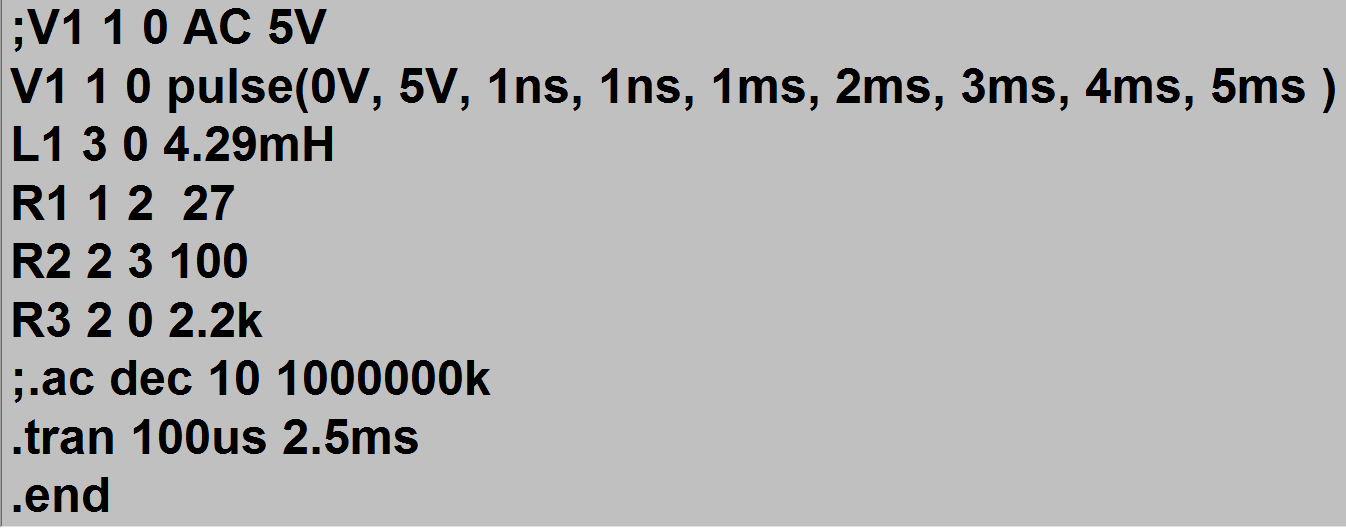
\includegraphics[scale=0.2]{cod}
	 	\caption{}
	 	\label{fig:cod}
	 \end{figure}
	 
	 \section{Resultados y Observaciones}
	 
	 \subsection{Análisis Transitorio}
	 Con los valores de $ R_1=27\Omega $, $ R_2=100\Omega $, $ R_3=2.2k\Omega $ y L=4.29mH. Al sustituir estos valores en la función de transferencia, se obtuvo:
	 
	 \begin{equation}
	 \frac{220k+9.438s}{282.1k+9.55383s}
	 \end{equation}
	 

Al tener nuestra función escalón una amplitud de 5V, se multiplica esta por 5, quedando:
\begin{equation}
\frac{1.11M+47.19s}{282.1K+9.55383s}
\end{equation}

Al sustituirse los valores en el código de Scilab, se obtiene:

\begin{figure}[H]
	\centering
	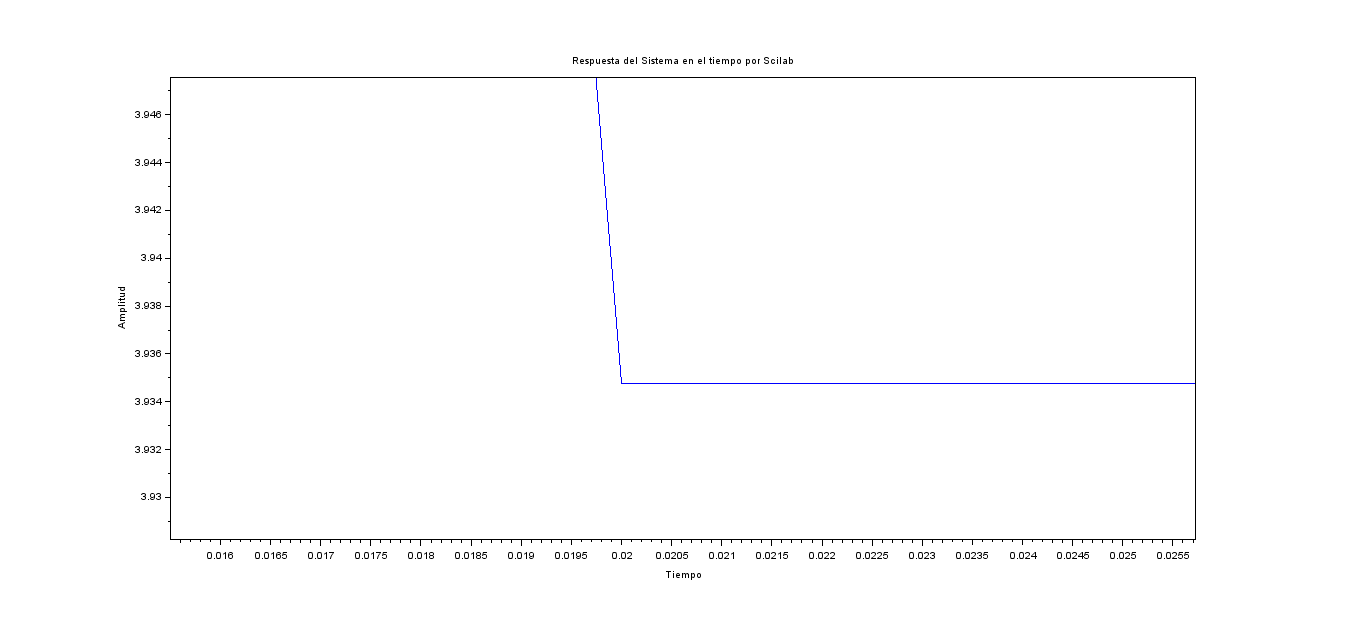
\includegraphics[scale=0.2]{trs.png}
	\centering
	\caption{Respuesta en el tiempo obtenida en Scilab}
	\label{trs}
\end{figure}

Y al simular en LTspice se obtuvo:

\begin{figure}[H]
	\centering
	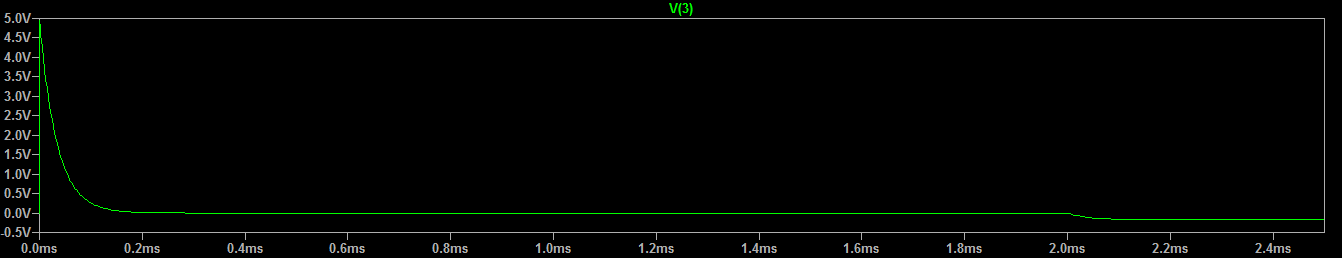
\includegraphics[width=0.7\linewidth]{trlt}
	\caption{Respuesta en el tiempo obtenida en LTSpice}
	\label{fig:trlt}
\end{figure}

El Tau de nuestra función de transferencia es igual a:
\begin{equation}
\tau=\frac{L}{R_2+R_1||R_3}=\frac{4.29mH}{126.67\Omega}=33.86\mu s
\end{equation}

A continuación se muestra el Tau en el circuito probado en el laboratorio:

\begin{figure}[H]
	\centering
	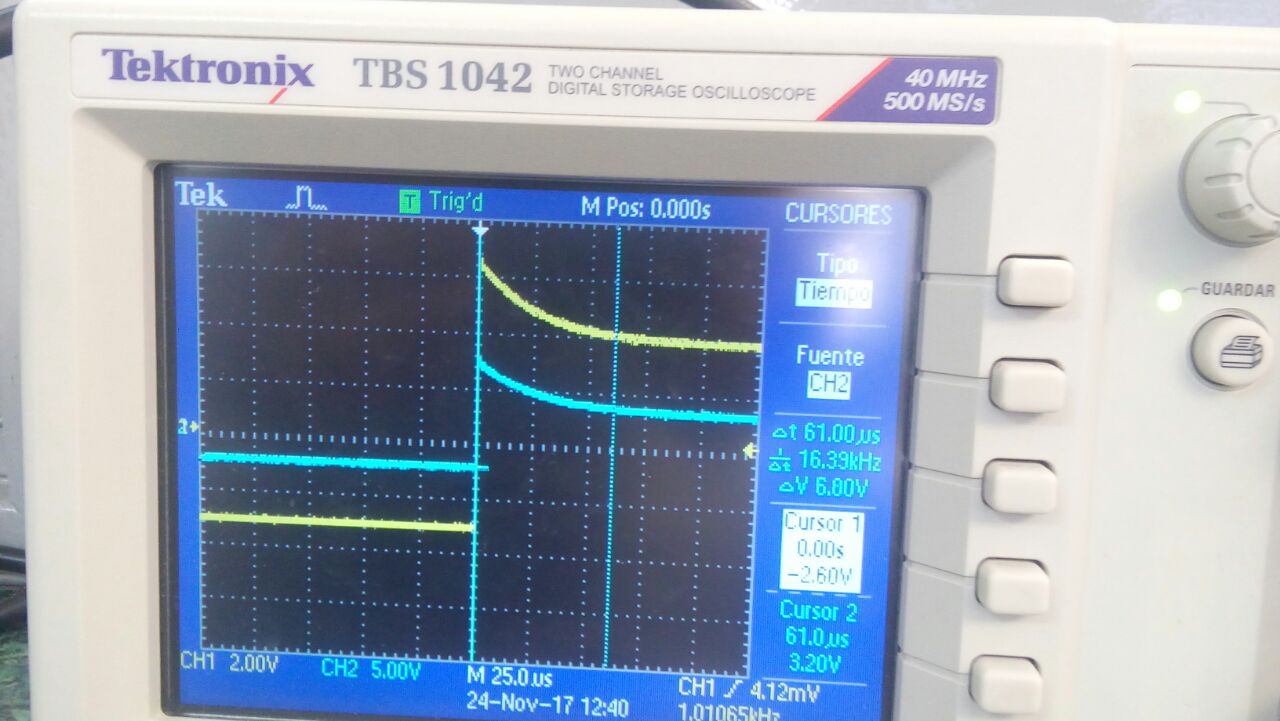
\includegraphics[width=0.7\linewidth]{tlab}
	\caption{Respuesta en el tiempo en el laboratorio.}
	\label{fig:tlab}
\end{figure}


\subsection{Barrido de Frecuencia}
A continuación se muestra el barrido de frecuencia obtenido al simular en LTspice, la amplitud de la señal senoidal como se puede ver en el código de LTspcie, es de 5V:

\begin{figure}[H]
	\centering
	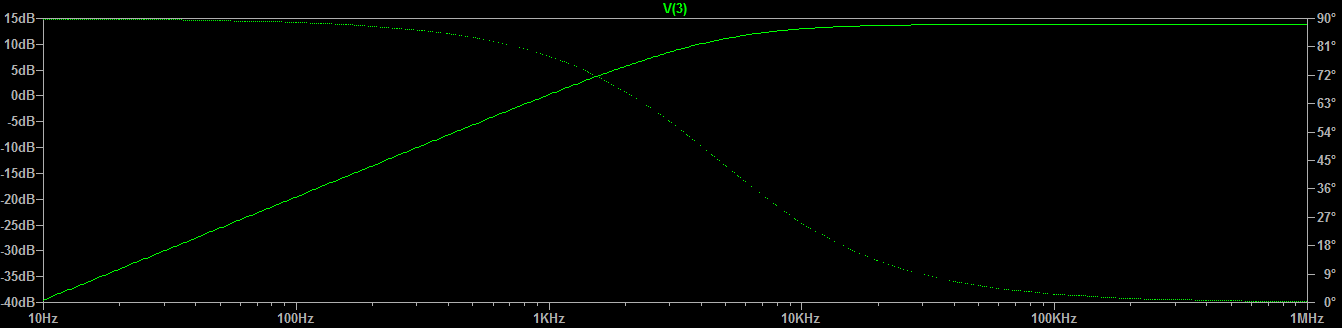
\includegraphics[width=0.7\linewidth]{frlt}
	\caption{Respuesta en frecuencia en LTspice}
	\label{fig:frlt}
\end{figure}

Posteriormente, se muestran los valores de voltaje obtenidos a distintas frecuencias obtenido en el laboratorio:

 \begin{table}[H]
	\centering
	\begin{tabular}{|l|c||}
		\hline
		\multicolumn{2}{|c|}{\textbf{Barrido en frecuencia}}\\
		\hline
		\textbf{Frecuencia (Hz)} & \textbf{Voltaje (V)} \\
		\hline
	10&	1.16\\
	20&	1.32\\
		\hline
	30&	1.36\\
		\hline
	40&	1.38\\
		\hline
	50&	1.36\\
		\hline
	60&	1.38\\
		\hline
	70&	1.35\\
		\hline
	80&	1.35\\
		\hline
	90&	1.35\\
		\hline
	100&	1.36\\
		\hline
	200	&1.37\\
		\hline
	300	&1.37\\
		\hline
	400&	1.38\\
		\hline
	500	&1.38\\
		\hline
	600&	1.38\\
		\hline
	700&	1.37\\
		\hline
	800&	1.36\\
		\hline
	900&	1.38\\
		\hline
	1000&	1.34\\
		\hline
	2000&	1.45\\
		\hline
	3000&	1.54\\
		\hline
	4000&	1.7\\
		\hline
	5000&	1.78\\
		\hline
	6000&	1.86\\
		\hline
	7000&	1.94\\
		\hline
	8000&	2.02\\
		\hline
	9000&	2.08\\
		\hline
	10000&	2.14\\
		\hline
	20000&	2.34\\
		\hline
	30000&	2.4	\\
		\hline
	40000&	2.4\\
		\hline
	50000&	2.42\\
		\hline
	60000&	2.42\\
		\hline
	70000&	2.44\\
		\hline
	80000&	2.44\\
		\hline
	90000&	2.44\\
		\hline
	100000&	2.44\\
		\hline
	200000&	2.44\\
		\hline
	300000&	2.46\\
		\hline
	400000&	2.44\\
		\hline
	500000&	2.44\\
		\hline
	600000&	2.42\\
		\hline
	700000&	2.42\\
		\hline
	800000&	2.4\\
		\hline
	900000&	2.4\\
		\hline
	1000000&	2.38\\
		\hline
		\end{tabular}
\end{table}

Y se grafican dichos valores en una escala semi-logarítmica: 

\begin{figure}[H]
	\centering
	\begin{tikzpicture}
	\begin{semilogxaxis}[xlabel=Frecuencia(Hz),ylabel=Voltaje de salida]
	\addplot [black] coordinates {
(	10,	1.16)
(	20,	1.32)
(	30,	1.36)
(	40,	1.38)
(	50,	1.36)
(	60,	1.38)
(	70,	1.35)
(	80,	1.35)
(	90,	1.35)
(	100	1.36)
(	200,	1.37)
(	300, 1.37)
(	400,	1.38)
(	500,	1.38)
(	600,	1.38)
(	700,	1.37)
(	800,	1.36)
(	900,	1.38)
(	1000,	1.34)
(	2000,	1.45)
(	3000,	1.54)
(	4000,	1.7)
(	5000,	1.78)
(	6000,	1.86)
(	7000,	1.94)
(	8000,	2.02)
(	9000,	2.08)
(	10000,	2.14)
(	20000,	2.34)
(	30000,	2.4)
(	40000,	2.4)
(	50000,	2.42)
(	60000,	2.42)
(	70000,	2.44)
(	80000,	2.44)
(	90000,	2.44)
(	100000,	2.44)
(	200000,	2.44)
(	300000,	2.46)
(	400000,	2.44)
(	500000,	2.44)
(	600000,	2.42)
(	700000,	2.42)
(	800000,	2.4)
(	900000,	2.4)
(	1000000,	2.38)
};  
	\end{semilogxaxis}
	\end{tikzpicture}
	\centering
	\caption{Gráfica de los valores de voltaje en función a la frecuencia.} 
\end{figure}


\subsection{Observaciones}
\textbf{Carlos Alberto Del Portillo Malandra:} 
Algo que se puede apreciar en el análisis transitorio es que los valores calculados y simulados difieren con lo medido, ya que a pesar de la resolución de la gráfica de Scilab se puede apreciar que el Tau se encuentra cercano al de LTspice y al calculado, se debió tener algún problema con inductor. En el análisis de frecuencia se obtuvo la forma de la gráfica como lo esperábamos, solo se tuve una pequeña diferencia al final pero pudo ser debido a las frecuencias a las que opera el inductor\\


\textbf{Gustavo Martínez Mondragón:} 
Se puede observar que en el análisis transitorio de nuestro circuito no coincide de con lo que se esperaba de los cálculos y lo simulado en LTspice, de igual forma, en el barrido de frecuencia al final se puede apreciar en la gráfica una pequeña pendiente negativa que no tiene la simulación, se puede deducir que los inductores que se ocuparon en el laboratorio no están hechos para altas frecuencias.

\section{Conclusiones}
\textbf{Carlos Alberto Del Portillo Malandra:} 
Al realizar la inspección del sistema encontrando sus polos y ceros y realizando una comparación de los resultados obtenidos mediante la simulación por Spice y al realizar el barrido de frecuencia en el circuito, podemos observar que los valores obtenidos por la simulación son mas precisos pudiendo apreciar la caída en el caso del inductor.\\

\textbf{Gustavo Martínez Mondragón:} 
Se puede apreciar a lo largo del desarrollo teórico que encontrar los elementos de nuestra función de transferencia es más fácil usando el método de inspección que el algebraico que se usa comúnmente, ya que este último es más laborioso y tardado por el método más sencillo (divisor de voltaje) y puede que al toparnos con sistemas más complejos, en este caso circuitos con más mallas, la mejor opción sea el método de inspección.

A su vez fue de gran ayuda el programa de LTspice ya que es muy simple, y los distintos análisis que nos ofrece nos ayudan a evaluar el comportamiento de nuestro sistema.
	
	
\end{document}